\documentclass{article} % For LaTeX2e
\usepackage{nips14submit_e,times}
\usepackage{hyperref}
\usepackage{url}
\usepackage{graphicx}
\usepackage{amsmath}
%\documentstyle[nips14submit_09,times,art10]{article} % For LaTeX 2.09


\title{Modeling Economic Network Resilience: Growth, Shock, and Recovery Dynamics}


\author{
Aditya Ranjan\thanks{ Fore code and all the figures, use my github link: } \\
Humanities and Social Science\\
Indian Institute of Technology\\
Roorkee, Uttarakhand 247667 \\
\texttt{a\_ranjan@hs.iitr.ac.in}
}



\newcommand{\fix}{\marginpar{FIX}}
\newcommand{\new}{\marginpar{NEW}}

\nipsfinalcopy % Uncomment for camera-ready version



\begin{document}

\maketitle

\begin{abstract}
This report presents the development and analysis of a multi-layered network model designed to simulate economic dynamics, including the effects of growth, financial shocks, and recovery processes. I began with a simple, randomly weighted network structure representing multiple interconnected industries or sectors, and gradually introduced economic growth and random changes. Over the course of the simulation, I applied a financial shock to observe its impact on the network's structure and followed it with a recovery phase to study the system's resilience. Key metrics such as Inverse Participation Ratio (IPR) and Eigenvector Centrality were used to analyze the changes in network structure at each stage. This report explores the evolution of these metrics across the different phases of the simulation, focusing on how the network adapts to internal and external disruptions. The findings provide insights into the adaptability, resilience, and centralization of economic networks in response to economic shocks and recovery mechanisms.
\end{abstract}

\section{Introduction}
Economic systems are complex, composed of interconnected entities such as industries, countries, or financial institutions, and are subject to dynamic changes driven by growth, crises, and recovery. Understanding these dynamics is crucial for developing resilient frameworks capable of withstanding and recovering from economic shocks.

Network theory has emerged as a powerful tool for modeling complex systems, representing economic relations where nodes are entities and edges represent interactions, such as trade or financial transactions. Network models capture both the structure and dynamics of economic systems, offering insights into power, influence, and vulnerability.

This report explores the evolution of a multi-layered economic network over time. It begins with the creation of a simple, randomly weighted network, incorporating random iterations to simulate unpredictable changes. The network evolves in stages, starting with steady economic growth and fluctuations, followed by a financial shock to simulate an economic crisis, and ending with a recovery phase. During each stage, random changes to the network structure, such as the addition and removal of edges, simulate real-world dynamics like trade policies or financial linkages.

In the final model, we also analyze the Clustering Coefficient, which measures how nodes cluster together. This helps us understand the interconnectedness within the network and the impact of disruptions on network structure. By examining Inverse Participation Ratio (IPR), Eigenvector Centrality, and Clustering Coefficient, this study provides a comprehensive view of how economic systems respond to growth, shocks, and recovery.

These network metrics help identify key changes in economic behavior over time, offering insights that are valuable for policymakers and economists seeking to design more resilient economic systems. Understanding how networks evolve in the face of growth, crisis, and recovery can inform decision-making and support long-term stability in interconnected systems.



\section{Methodology}
The methodology for this study involves simulating the evolution of a multi-layered economic network over a 30-year period, beginning with a basic random network and evolving it through various stages. Each stage represents a different phase in the economic system's development, including steady growth, a financial shock, and a recovery phase. The analysis focuses on the network metrics Inverse Participation Ratio (IPR), Eigenvector Centrality, and Clustering Coefficient to observe the structural changes in the network and to understand how economic conditions affect the system. The network models were created and analyzed step by step as described below:


\subsection{Creation of the Initial Network}
The initial step involved the creation of a simple, randomly weighted multi-layered network with 20 nodes in each of the two layers. Each layer represented a different industry or sector, and the nodes represented individual entities within these sectors, such as countries or industries. The edges between nodes represented economic ties such as trade or financial relationships.

The edges were assigned weights based on a normal distribution with a mean (\(\mu\)) of 50 and a standard deviation (\(\sigma\)) of 10. The network was created with random connections between the nodes, and self-loops (edges that connect a node to itself) were also added with a 30\% chance. The initial network was designed to be a directed graph, where the direction of the edges indicated the flow of economic activity between nodes.
\begin{figure}[h]
\begin{center}
    \includegraphics[width=0.7\textwidth]{"Multilayered network.png"}
\end{center}
\caption{Network graph showing trade connections between industries.}
\end{figure}

The primary network metrics used in this analysis are:
\begin{itemize}
  \item \textbf{Eigenvector Centrality}: Calculated as the principal eigenvector of the adjacency matrix of the network:
  \[
  \mathbf{Ax} = \lambda \mathbf{x}
  \]
  \item \textbf{Clustering Coefficient}: Given by:
  \[
  C_i = \frac{2e_i}{k_i(k_i - 1)}
  \]
  where \( e_i \) is the number of edges between the neighbors of node \(i\) and \( k_i \) is the degree of node \(i\).
  \item \textbf{Inverse Participation Ratio (IPR)}: Calculated as:
  \[
  \text{IPR} = \sum_i c_i^4
  \]
  where \( c_i \) is the eigenvector centrality of node \(i\).
\end{itemize}

\subsection{Random Iterations}
Once the network was established, the network was recreated 30 times. In each iteration, the nodes and edges were randomized to ensure that the network structure varied with each run. This approach aimed to generate multiple network configurations, making the analysis more robust and less sensitive to any specific network layout.

For each recreated network, the Inverse Participation Ratio (IPR) was calculated to assess how concentrated the eigenvector centrality was across the network. The IPR is defined as the sum of the fourth powers of the eigenvector centralities of all nodes, which gives an indication of the distribution of centrality in the network. A higher IPR indicates that a few nodes dominate the network's centrality, while a lower IPR suggests a more even distribution of influence.

In addition to IPR, the eigenvector centrality of all nodes was also computed for each random iteration. This centrality measure assesses the influence of each node based on both the number and quality of its connections, considering the centrality of its neighbors. Eigenvector centrality was tracked over all iterations, and the evolution of the centrality for individual nodes was plotted for both layers of the network.

\subsection{Economic Growth Simulation}

To simulate steady economic growth, each node in the network, representing an economic entity, starts with an initial growth value of 1.0. Annually, each node’s growth is updated by a rate of 2\%, with a slight fluctuation of 0.5\%, to reflect consistent yet realistic growth. The update formula is as follows:

\begin{equation}
\text{new growth} = \text{current growth} \times (1 + \text{growth rate})
\end{equation}

Edge weights, representing interaction strengths, are adjusted based on the economic growth of connected nodes, with a 3\% growth factor applied:

\begin{equation}
\text{new weight} = \text{current weight} \times \left(1 + 0.03 \times \frac{\text{growth}_{\text{node}} + \text{growth}_{\text{neighbor}}}{2}\right)
\end{equation}

To mimic real-world dynamics, edges have a 1\% chance of removal and a 3\% chance of formation each year, simulating changing economic ties. These mechanisms provide a basis to assess how gradual economic growth impacts network metrics like eigenvector centrality and Inverse Participation Ratio (IPR), setting up a foundation for later stages involving shocks and recovery analysis.



\subsection{Economic Shock Simulation}

To explore the effects of a financial shock on network dynamics, we introduced a severe economic downturn at year 18. In this model, each inter-nodal connection, represented by directed weighted edges, experienced a 70\% reduction in weight, simulating a sudden contraction in economic activity. The shock was applied globally across all edges, which reflects a widespread financial crisis scenario impacting all interconnected entities.

Following the shock, network metrics, including eigenvector centrality and the Inverse Participation Ratio (IPR), were recalculated to evaluate the structural impact of this disruption on network stability and node influence. These metrics allowed us to observe changes in the prominence of highly connected nodes and shifts in the concentration of network influence.




\subsection{Shock and Recovery Mechanism}
To capture the effects of economic shocks and recovery, we introduced a significant financial shock at year 18, reducing edge weights by 70\% to reflect a sudden decrease in inter-country interactions. The network was then evolved through a two-year cool-down period, during which edge weights were gradually increased to simulate recovery. After recovery, a slight decentralization was introduced, reducing edge weights by 2\% annually, to model long-term shifts in economic structure.

Throughout these phases, we tracked changes in the \textit{Inverse Participation Ratio (IPR)} to measure network concentration and \textit{eigenvector centrality} for individual node influence, visualizing the impact of shock and recovery on network stability and resilience.




\subsection{Clustering Coefficient Dynamics}

To capture the evolution of local network cohesion, we computed the \textit{clustering coefficient} at each year of the simulation. The clustering coefficient reflects the degree to which nodes in the network tend to cluster together, providing insights into the strength of local connections. During the steady economic growth phase, the clustering coefficient remained stable, indicating consistent local interconnections. 

However, following the financial shock at year 18, the clustering coefficient decreased, reflecting weakened connectivity due to reduced edge weights. As the network underwent recovery during the subsequent cool-down period, the clustering coefficient gradually increased, demonstrating the re-establishment of interconnections within the network. After the recovery phase, a gradual decentralization of the network structure was observed, as edge weights decreased by 2\% annually, which led to a slow but steady reduction in the clustering coefficient, capturing long-term shifts in network cohesion.


\section{Discussion}

\subsection{Random Iterations: IPR}

\begin{figure}[h]
\begin{center}
    \includegraphics[width=0.7\textwidth]{"Random IPR.png"}
\end{center}
\caption{IPR for random iterations 30 times.}
\end{figure}
\textbf{Graph Description:} The graph displays the IPR values across 30 random iterations of the same network.

\textbf{Observation:} The IPR fluctuates within a narrow range, remaining between approximately 0.0253 and 0.0257. This indicates minor variations with no clear upward or downward trend.

\textbf{Inference:} These fluctuations suggest that random reconfigurations of the network do not significantly alter its structural concentration. The IPR remains relatively stable, implying that the random variations do not change the network’s overall influence distribution among nodes.


\subsection{Steady Growth with Minor Fluctuations: IPR}
\begin{figure}[h]
\begin{center}
    \includegraphics[width=0.7\textwidth]{"IPR steady growth.png"}
\end{center}
\caption{IPR with steady growth rate at 2\%.}
\end{figure}

\textbf{Graph Description:} The graph shows the IPR evolving over 30 years under a steady growth rate with minor fluctuations.

\textbf{Observation:} The IPR exhibits a steady upward trend, starting around 0.12 and gradually increasing to over 0.22 by year 30.

\textbf{Inference:} This trend suggests that, as the network grows, certain nodes become more dominant, leading to a more centralized or concentrated structure. The increase in IPR reflects a rise in participation concentration, meaning that influence within the network is becoming more focused on fewer nodes over time. The minor fluctuations represent small disturbances, but the steady growth indicates a consistent trend toward centralization.

\subsection{Shock and Recovery: IPR}
\begin{figure}[h]
\begin{center}
    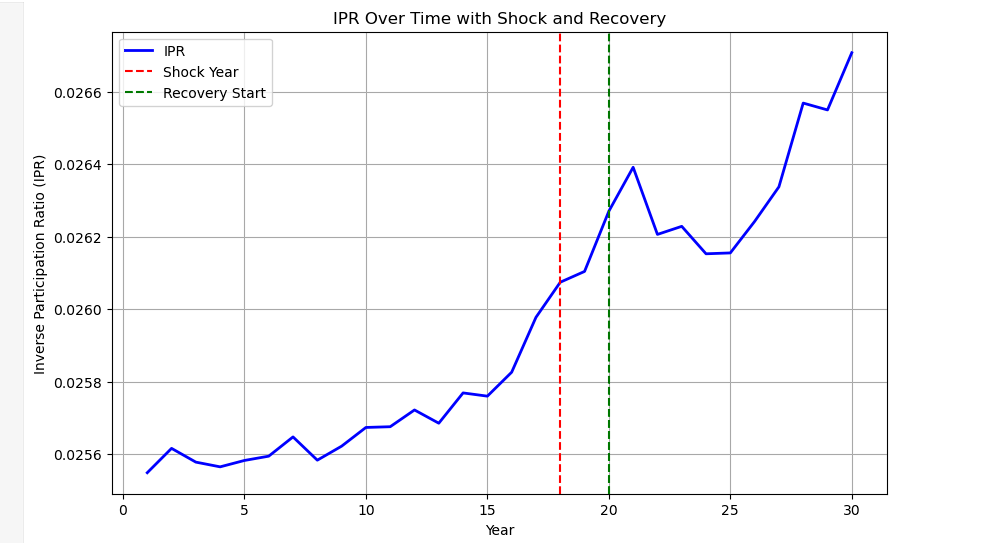
\includegraphics[width=0.7\textwidth]{IPR with shock and Recovery.png}
\end{center}
\caption{IPR for simulation with shock and recovery.}
\end{figure}
\textbf{Graph Description:} The graph illustrates the IPR evolution over 30 years, with a shock applied at year 18 (red vertical line) and a recovery period starting at year 20 (green vertical line).

\textbf{Observation:}

\begin{itemize}
    \item \textbf{Years 0--17:} The IPR steadily increases, similar to the steady growth scenario, indicating gradual centralization in the network structure.
    \item \textbf{Shock at Year 18:} At this point, there is a noticeable rise in the IPR, suggesting that the shock further concentrates influence within the network. Instead of a drop, the IPR spikes, which may mean the shock amplifies the influence of already dominant nodes or reduces the influence of less connected nodes.
    \item \textbf{Recovery from Year 20 Onwards:} After the shock, the IPR continues to grow steadily with minor fluctuations, reaching new highs by year 30. This phase indicates that, rather than dispersing influence, the recovery process actually reinforces the centralization trend.
\end{itemize}

\textbf{Inference:} The shock, instead of redistributing influence or decentralizing the network, accelerates the process of concentration, making the network even more hierarchical. The recovery period seems to further enhance this centralization, possibly as the network reorganizes to strengthen the existing influence structure among key nodes.





\subsection{Random Iteration in the Absence of Economic Influences}
\begin{figure}[h]
\begin{center}
    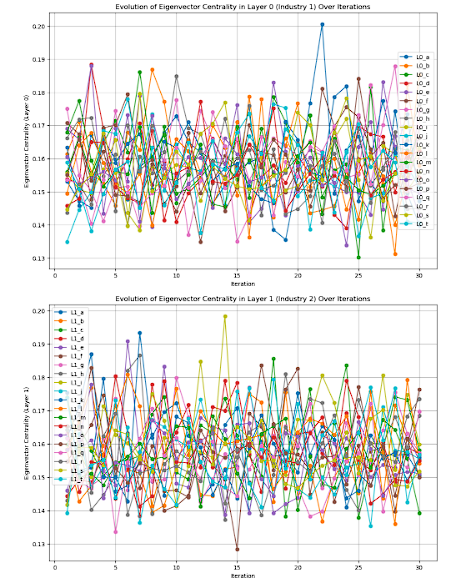
\includegraphics[width=0.7\textwidth]{Random EC.png}
\end{center}
\caption{Eigenvector centrality for random iterations 30 times.}
\end{figure}

In the first scenario, eigenvector centrality was analyzed without any economic influence. The centrality trajectories across both layers exhibit random fluctuations over 30 years, with no discernible upward or downward trend. This behavior suggests that, in the absence of systematic economic growth or shocks, the importance of nodes within the network remains volatile and unpredictable. The fluctuations reflect the inherent randomness in node interactions when no external stabilizing factors are applied.


\subsection{Steady Economic Growth of 2\% with 0.5\% Fluctuation}



The second scenario incorporates a steady economic growth rate of 2\%, with a fluctuation margin of $\pm0.5\%$ over 30 years. Under this condition, eigenvector centrality evolves more predictably, with a general trend of increasing centrality values for certain nodes. In \textit{Layer 0}, nodes exhibit gradual and differentiated growth in centrality, likely reflecting varying levels of connectivity and influence within the layer. \textit{Layer 1} shows a similar growth pattern, but with some nodes achieving consistently higher centrality values, suggesting greater influence or connectivity within this layer. This observation underscores the stabilizing effect of steady economic growth on node importance, as certain nodes become more central within the network structure.
    \begin{figure}[h]
    \begin{center}
        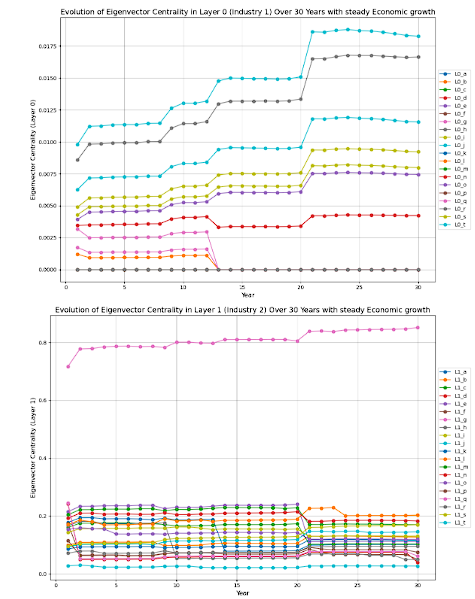
\includegraphics[width=0.7\textwidth]{Growth EC.png}
    \end{center}
    \caption{Eigenvector centrality with steady growth.}
    \end{figure}


\subsection{Impact of Economic Shock at Year 18 with Recovery by Year 20}

\begin{figure}[h]
\begin{center}
    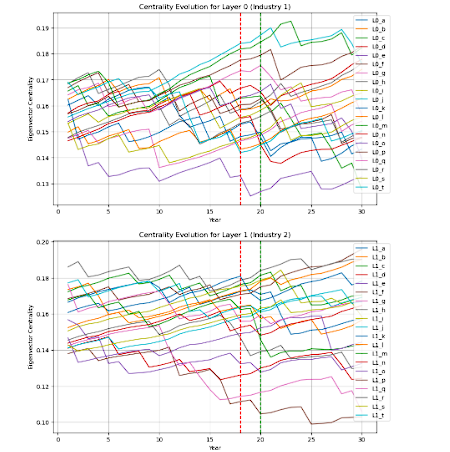
\includegraphics[width=0.7\textwidth]{Shock and recovery EC.png}
\end{center}
\caption{Eigenvector centrality with shock and recovery.}
\end{figure}

The third scenario examines the effects of an economic shock applied at year 18, followed by a recovery phase starting at year 20. The shock introduces significant volatility in the centrality values, disrupting the previously stable growth patterns observed during steady economic conditions. Several nodes experience a marked decrease in centrality during the shock period, indicating reduced influence within the network. Post-recovery, while centrality values attempt to realign with pre-shock levels, they do not completely revert to the original trajectory, highlighting the lasting impact of economic disruptions on network structure. This result suggests that although recovery efforts help stabilize the network, they may not fully mitigate the long-term effects of economic shocks on node centrality.

Overall, these findings highlight the sensitivity of network structure to external economic factors. Steady growth promotes gradual and stable increases in centrality, while economic shocks create immediate and sometimes lasting disruptions in node importance.


\subsection{Decline in Clustering Coefficient Post-Economic Shock}


\begin{figure}[h]
    \begin{center}
        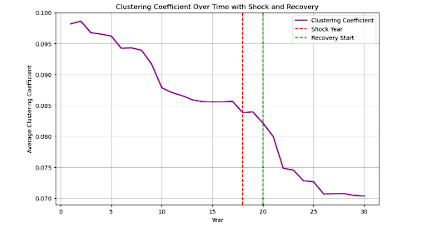
\includegraphics[width=0.7\textwidth]{Clustering coefficient.png}
    \end{center}
    \caption{clustering coefficient over time with shock and recovery.}
    \end{figure} 
The analysis of the clustering coefficient in the third scenario, where an economic shock is introduced at year 18 followed by recovery at year 20, reveals a steady decline in clustering over time. This trend suggests that the network’s structural cohesion is compromised due to the shock. Specifically, the decline in the clustering coefficient indicates a reduction in the local interconnectedness of nodes, meaning fewer nodes participate in tightly knit clusters.

This reduction in clustering implies that the shock weakened certain relationships within the network, potentially isolating nodes and reducing the overall cohesiveness of the network structure. Although a recovery phase begins at year 20, the clustering coefficient does not return to pre-shock levels, suggesting a lasting impact of the shock. Some connections lost during the shock period may not have been re-established, resulting in a permanently altered, less cohesive network.

This decline in clustering highlights a vulnerability in the network's resilience. A lower clustering coefficient reduces the presence of redundant connections, making the network more susceptible to future shocks or disruptions. In this state, the network may shift towards a more hierarchical or less interconnected structure, where nodes depend on fewer critical pathways, increasing the potential fragility of the network over time.





\section{Conclusion}
This study developed and analyzed a multi-layered economic network model to explore the impacts of growth, shocks, and recovery on network structure and resilience. The findings reveal that steady growth encourages a gradual centralization of influence within the network, as reflected by increasing Eigenvector Centrality and IPR. However, the introduction of an economic shock disrupts this trend, causing immediate volatility and structural changes. Recovery efforts only partially restore the network's original structure, indicating a lasting impact on connectivity and clustering.

By examining metrics such as Eigenvector Centrality, IPR, and Clustering Coefficient, this report provides insights into the adaptability and vulnerability of economic networks in response to external disruptions. The model suggests that while growth can reinforce network stability, shocks may induce lasting structural shifts, potentially reducing resilience. These findings underscore the importance of building redundancy and flexibility into economic systems to mitigate the long-term effects of crises.

\section{References}
\begin{thebibliography}{99}
\bibitem{Newman2010} Newman, M. E. J. (2010). \textit{Networks: An Introduction}. Oxford University Press.
\bibitem{Barabasi2002} Barabási, A.-L. (2002). \textit{Linked: The New Science of Networks}. Perseus Publishing.
\bibitem{Wasserman1994} Wasserman, S., \& Faust, K. (1994). \textit{Social Network Analysis: Methods and Applications}. Cambridge University Press.
\bibitem{Garlaschelli2004} Garlaschelli, D., \& Loffredo, M. I. (2004). Structure and evolution of the World Trade Network. \textit{Physical Review Letters}, 93(18), 188701.
\end{thebibliography}

\end{document}
